\documentclass[border=3pt]{standalone}
\usepackage{tikz}
\usepackage[scaled]{helvet}\renewcommand{\familydefault}{\sfdefault}
\usepackage[T1]{fontenc}
\usetikzlibrary{positioning,arrows.meta,calc}
\definecolor{orng}{HTML}{E69F00}\definecolor{blu}{HTML}{0072B2}\definecolor{grn}{HTML}{009E73}\definecolor{red}{HTML}{D55E00}
\begin{document}
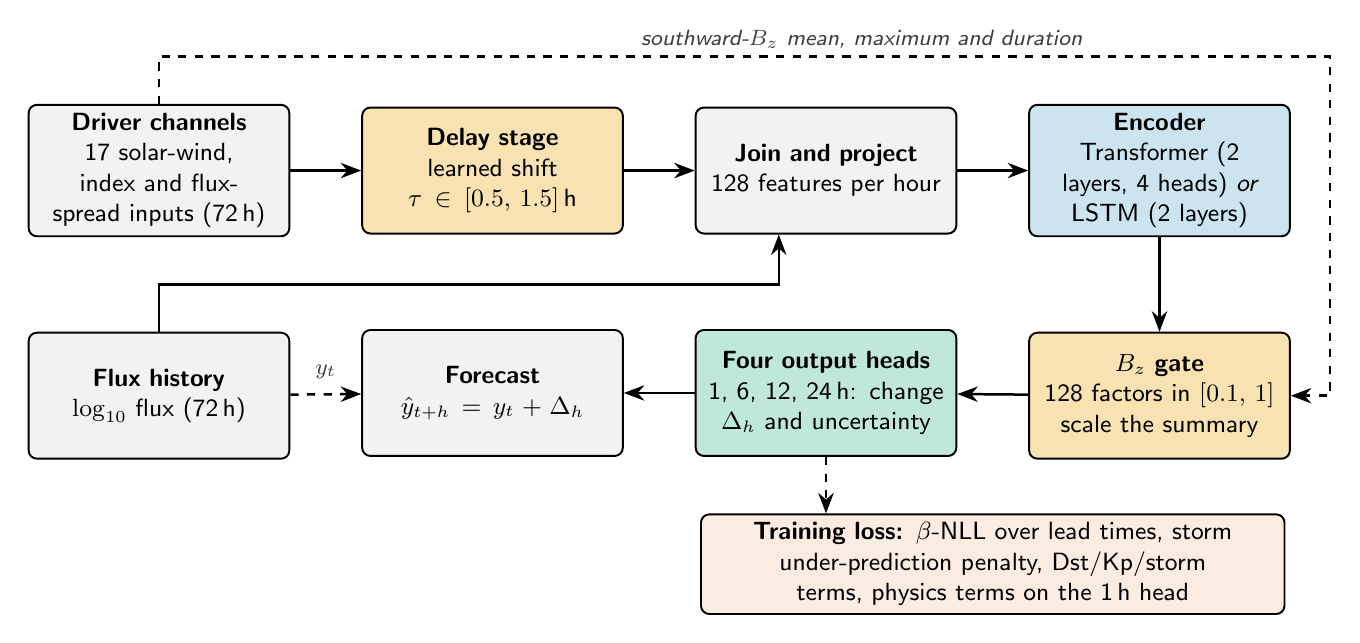
\begin{tikzpicture}[font=\small, node distance=12mm and 9mm,
  box/.style={draw, rounded corners=3pt, align=center, minimum height=16mm, text width=31mm, inner sep=3pt, line width=0.7pt},
  ar/.style={-{Stealth[length=2.6mm]}, line width=0.9pt}, lab/.style={font=\footnotesize\itshape, text=black!75, fill=white, inner sep=1pt}]
\node[box, fill=gray!10] (aux) {\textbf{Driver channels}\\17 solar-wind, index and flux-spread inputs (72\,h)};
\node[box, fill=orng!30, right=of aux] (delay) {\textbf{Delay stage}\\learned shift\\\(\tau\in[0.5,\,1.5]\)\,h};
\node[box, fill=gray!10, right=of delay] (proj) {\textbf{Join and project}\\128 features per hour};
\node[box, fill=blu!20, right=of proj] (enc) {\textbf{Encoder}\\Transformer (2 layers, 4 heads) \emph{or} LSTM (2 layers)};
\node[box, fill=gray!10, below=of aux] (flux) {\textbf{Flux history}\\\(\log_{10}\) flux (72\,h)};
\node[box, fill=gray!10, below=of delay] (out) {\textbf{Forecast}\\\(\hat y_{t+h}=y_t+\Delta_h\)};
\node[box, fill=grn!25, below=of proj] (heads) {\textbf{Four output heads}\\1, 6, 12, 24\,h: change \(\Delta_h\) and uncertainty};
\node[box, fill=orng!30, below=of enc] (gate) {\(\boldsymbol{B_z}\) \textbf{gate}\\128 factors in \([0.1,\,1]\) scale the summary};
\node[box, fill=red!12, below=7mm of $(heads.south)!0.5!(gate.south)$, anchor=north, text width=72mm, minimum height=11mm] (loss)
  {\textbf{Training loss:} \(\beta\)-NLL over lead times, storm under-prediction penalty, Dst/Kp/storm terms, physics terms on the 1\,h head};
\draw[ar] (aux) -- (delay); \draw[ar] (delay) -- (proj); \draw[ar] (proj) -- (enc);
\draw[ar] (enc) -- (gate); \draw[ar] (gate) -- (heads); \draw[ar] (heads) -- (out);
\draw[ar] (flux.north) -- ++(0,6mm) -| ([xshift=-6mm]proj.south);
\draw[ar, dashed] (flux) -- node[lab, above=1.5mm] {\(y_t\)} (out);
\draw[ar, dashed] (aux.north) -- ++(0,6mm) -| node[lab, pos=0.3, above=0.5mm] {southward-\(B_z\) mean, maximum and duration} ([xshift=5mm]enc.east) |- (gate.east);
\draw[ar, dashed] (heads.south) -- (heads.south |- loss.north);
\end{tikzpicture}
\end{document}
